\documentclass[10pt,a4paper]{article}
\usepackage[utf8]{inputenc}
\usepackage[spanish]{babel}
\usepackage{amsmath}
\usepackage{amsfonts}
\usepackage{amssymb}
\usepackage{graphicx}
\usepackage{listings}
\usepackage{subfig}
\usepackage{hyperref}
\usepackage{float}
\selectlanguage{spanish} 
\usepackage[spanish,onelanguage,linesnumbered,algoruled,boxed,lined]{algorithm2e} %for psuedo code

\usepackage[left=2cm,right=2cm,top=2cm,bottom=2cm]{geometry}
\usepackage{endnotes}


\begin{document}

\title{Cómputo Paralelo\\Proyecto I}
\author{Jose Antonio Gallardo Monroy}

\maketitle

\section{Introducción}

\noindent En este proyecto se ataca el problema de asignación de frecuencias utilizando algoritmos genéticos. Específicamente, se implementa un algoritmo memético con control de diversidad. La parte correspondiente a cómputo paralelo es realizar las búsquedas locales al mismo tiempo con múltiples núcleos; se utiliza MPI para comunicarse entre diferentes núcleos $c-1-i$ del \textit{cluster El insurgente} utilizando las funciones $MPI\_Send$ y $MPI\_Recv$.


\section{Planteamiendo del problema}

\noindent Asociado al problema de asignación de frecuencias, se tiene un grafo $G(V, E)$ con $N$ nodos numerados de $0$ a $N-1$ y $|E|$ aristas; los nodos representan a los transmisores y las aristas una posible interferencia entre esos transmisores. Además del número de transmisores se tiene un número de canales $K$; cada transmisor debe utilizar un canal. Una asignación es una función $f:V \rightarrow  \{0, 1, \dots, K-1 \}$.

\noindent Para determinar si hay interferencia, se tiene una función $g: E \rightarrow I\!\!N_0 \times I\!\!N$. Dado un arista $x \in E$ que une a los vértices $u_x$ y $v_x$, $g(x)_0$ representa el rango en el cual hay interferencia. Dada una asignación $f(\cdot)$, si

\begin{equation*}
| f(u_x) - f(v_x) | \leq g(x)_0 
\end{equation*}

\noindent hay interferencia entre ambos transmisores. Dicha interferencia es penalizada con $g(x)_1$ unidades. Por tanto, se quiere minimizar

\begin{equation*}
\sum_{x \in E} 1\left[ | f(u_x) - f(v_x) | \leq g(x)_0 \right] \cdot g(x)_1, 
\end{equation*}

\noindent donde $1 ( \cdot )$ es la función indicadora.

\section{Metodología}

\noindent Se toma como referencia el artículo de Carlos Segura et al titulado \textit{Improving Diversity in EAs: New Best Solutions for Frecuency Assignment}. Se implementa un algoritmo memético con control de diversidad. Cabe aclarar que no se implementa de manera exacta al artículo, la implementación realizada es mucho más sencilla.

\subsection*{Búsqueda local}

\noindent La búsqueda local se realiza a fuerza bruta sobre los vecinos de la asignación $f(\cdot)$. La vecindad de $f(\cdot)$ corresponde al conjunto de funciones que resultan de modificar la asignación de un transmisor por cualquier otro canal, es decir, cada elemento tiene $NK - 1$ vecinos (excluyendo a él mismo). Se toma una permutación aleatoria de los vértices y se exploran las asignaciones en ese orden, al encontrar un vecino con mejor evaluación, se avanza en esa dirección y se repite el proceso con otra permutación. 

\noindent Se puede calcular el costo que tiene una asignación $f( \cdot )$ recorriendo las aristas $E$ del grafo $G$. Al hacer la búsqueda local no se recorren todas las aristas, al cambiar la asignación $f(u)$ y conocer su costo, es posible conocer el costo de la nueva asignación consultando los vecinos de $u$; así, la complejidad es lineal sobre el número de vecinos que tiene el nodo que está siendo modificado, que es menor o igual al número de aristas.

\subsection*{Operadores}

\noindent Se define de manera arbitraria un natural $R$. Para el operador de mutación, se construye una lista $U$ con un vértice $u$ seleccionado de manera aleatoria. Lo siguiente se repite $r$ veces, con $r$ un número aleatorio entre $1$ y $R$ (incluídos): se toma un vértice $v$ de manera aleatoria de la lista $U$, se modifica de manera aleatoria; se buscan los vértices que tienen conflicto con la nueva asignación de $v$, se añaden a la lista $U$ y son modificados de manera aleatoria con probabilidad $Pm$. 

\noindent La cruza es análoga a la mutación. Dadas dos asignaciones $f(\cdot)$ y $g(\cdot)$, se contruye una lista $U$ con un vértice $u$ seleccionado de manera aleatoria. Lo siguiente se repite $r$ veces tomando la asignación $f(\cdot)$, con $r$ un número aleatorio entre $1$ y $R$ (incluídos): se toma un vértice $v$ de manera aleatoria de la lista $U$ pero no se modifica; se buscan los vértices que tienen conflicto con $v$ y se añaden a la lista $U$. Después de iterar $r$ veces, se define al hijo como una asignación

\begin{equation*}
h(x)= \left\{ \begin{array}{lcc}
             g(x) &   si  & x \in U  \\
             \\ f(x) & en\ otro\ caso &
             \end{array}
   \right.
\end{equation*}

\subsection*{Búsqueda local iterada}

\noindent Se define un número de iteraciones $BI\_n$ y se realiza lo siguiente $BI\_n$ veces: se perturba la asignación $f(\cdot)$ con la mutación descrita anteriormente y se realiza una búsqueda local; después de la búsqueda local se conserva la mejor asignación entre la que se tenía antes de ser perturbada y la que se obtuvo después de perturbar y hacer la búsqueda local.

\subsection*{Algoritmo memético}

\noindent El esquema que se sigue es el siguiente:

\begin{algorithm}[H] %or another one check
\caption{Algoritmo Memético} 
\label{algoritmo1}
%\KwIn{Un grafo }
%\KwOut{Mínimo tiempo requerido para realizar $nodo$. }
\SetAlgoLined

Inicializar población.\\
Mejorar cada individuo de la población con una búsqueda local iterada.\\

\While { No se cumpla criterio de paro} { \label{parar}

	Seleccionar a la mitad de los individuos por medio de un torneo. \\
	Crecer la población cuatro veces usando operadores. \\ \label{operadores}
	Realizar búsqueda local iterada por cada individuo en la población. \\
	Seleccionar la mitad de los individuos por torneo o por control de diversidad. \label{opcion}

}

\Return{Mejor individuo encontrado}

\end{algorithm}

\ \\

\noindent Los individuos se inicializan tomando muestras de una variable discreta que se distribuye de manera uniforme en los enteros $\{0, 1, \dots, k-1 \}$.

\noindent La ejecución del algoritmo se realiza durante un tiempo determinado, en la linea \ref{parar}, el tiempo de ejecución es el criterio de paro, es decir, se especifica el tiempo que correrá el algoritmo y después de ese tiempo, la próxima vez que se evalúe la condición se sale del ciclo \textit{while}.

\noindent La población es de tamaño $50$. En la linea \ref{operadores}, hay $25$ individuos de la población; primeramente se incrementa a $50$, añadiendo mutaciones de los $25$ individuos, después, se agregan $50$ individuos cruzando los $50$ que ya estaban (primeros $25$ con sus mutaciones). En la linea \ref{opcion} hay $100$ individuos, después se reduce a la mitad por medio de un torneo o por un medio de control de diversidad.

\subsubsection*{Selección por torneo}

\noindent Siempre se conserva al mejor individuo. Se permutan los individuos de manera aleatoria y se agrupan en parejas, la probabilidad de elegir al mejor se fija en $0{.}65$. Previamente se calculan los costos de todos los individuos, por ello, se sabe quién es el mejor individuo; si uno de los dos individuos es el mejor de todos, no se decide a quien conservar de manera aleatoria, se pasa automáticamente al mejor individuo; si ninguno de los dos es el mejor individuo, se conserva al mejor con probabilidad $0{.}65$.

\subsubsection*{Selección por diversidad}

\noindent Siempre se conserva al mejor individuo. Se trata de tener diversidad entre los individuos con la intención de evitar convergencia prematura y explorar mejor el espacio de búsqueda. Para hablar de diversidad, se utiliza una métrica, en este caso, se toma la distancia de \textit{Hamming} normalizada:

\begin{equation*}
d(f, g) = \dfrac{1}{N} \cdot \sum_{i=1}^N 1 \left( f(i) = g(i) \right).
\end{equation*} 

\noindent Al tener una métrica, se tiene una referencia de cercanía y lejanía. Para que haya diversidad, se busca que los individuos estén lejos los unos de los otros. Al inicio del programa, se busca que los individuos esten dispersos, pero conforme transcurre el tiempo se pide menos diversidad. El algoritmo de selección es el siguiente:

\ \\

\begin{algorithm}[H] %or another one check
\caption{Selección por diversidad} 
\label{algoritmo2}
\KwIn{Poblcion}
\KwOut{NuevaPoblacion}
\SetAlgoLined

$NuevaPoblacion = \{ MejorIndividuo(Poblacion) \}$ \\
Eliminar al mejor individuo de la población. \\
$D(tiempo) \leftarrow $ distancia mínima deseada entre todas las parejas de individuos. \\ \label{tiempo}


\While { No haya suficientes individuos en $NuevaPoblacion$} { 

	\For{$x \in Poblacion$} {
		$x.d \leftarrow $ distancia al individuo más cercano en $NuevaPoblacion$ \label{distancias}
		
		\If{$x.d < D$} {
			$x.costo \leftarrow \infty$		
		
		}		
		
	}

	$ND \leftarrow$ elementos no domindos en $Poblacion$ minimizando el costo y maximizando la distancia. \\
	$x \leftarrow $ Un individuo de $ND$ tomado de manera aleatoria. \\
	Se agrega $x$ a $NuevaPoblacion$.\\
	$x$ es eliminado de $Poblacion$.
	


}

\Return{NuevaPoblacion}

\end{algorithm}

\ \\

\noindent En la linea \ref{tiempo} el tiempo determina el valor de $D$. Se recibe como parámetro el tiempo de ejecución total $T_f$ y la distancia inicial $D_i$. Si se llega a dicha linea en el tiempo $T_a$, se hace

\begin{equation*}
D = D_i - D_i \cdot \dfrac{T_a}{T_f}.
\end{equation*}

\noindent Se pide una distancia $D_i$ entre todos los individuos y aquél que no tenga una distancia mayor será penalizado y no importará el costo que tenga, así, aquellos individuos que sí sean diversos se verán beneficiados y serán tomados en cuenta para la nueva población.

\section{Implementación}

\noindent Hay dos implementaciones, una secuencial y una paralela. La paralela se basa en la secuencial y use el esquema maestro-esclvo; el maestro tiene el control del memético y reparte las búsquedas locales iteradas entre los esclavos, al terminar, los esclavos regresan las soluciones y el maestro sigue con el algoritmo. Se utilizó MPI de manéra muy similar a la tarea del conjunto de \textit{Mandelbrot}.

\noindent  En la linea \ref{distancias} del Algoritmo \ref{algoritmo2}, se calculan distancias entre individuos de la población y la nueva población; se observa que si un individuo de la población no es seleccionado para la nueva población, en la siguiente iteración se necesitan nuevamente las distancias. Para no calcular dos veces la misma distancia, se almacenan las distancias ya calculadas en una tabla. 

\noindent Los individuos no dominados se encuentran en $O\left(n^2\right)$, se sabe que se pueden encontrar en $O(n log(n))$, pero $n = 50$, así que se prefiere usar un algoritmo cuadrático. 

\noindent A decir verdad, excepto por la tabla que almacena las distancias, el resto de la implementación es \textit{straightforward}.


\section{Resultados}

\noindent Los programas se corrieron en \textit{El Insurgente}. El tiempo de ejecución fue de $24$ horas ($1440$ minutos). En el artículo de Segura et al, se hace $D_i = 0{.}75 N$, como se está normalizando la distancia (se divide entre $N$), se toma $D_i = 0{.}75$. La población es de $50$ individuos; se toma $R = 8$; la probabilidad de mutación se fija en $0{.}02$; la probabilidad de seleccionar al mejor individuo entre dos individuos en un torneo es de $0{.}75$ y en la búsqueda iterada se hacen $BI\_n = 200$ iteraciones. Los experimentos se realizan con el grafo GSM2-227, para más detalle del conjunto véase \textit{Lower Bounds for Fixed Spectrum Frequency Assignment}, de R Montemanni et al.

\noindent Primeramente, se toma $K = 29$. Se realizaron $18$ ejecuciones, $9$ con selección por torneo y $9$ con selección por diversidad, a continuación se presenta una tabla:


\begin{table}[H]
\centering
\begin{tabular}{|l|l|l|l|}
\hline
Estrategia & Promedio & Mínimo & Máximo \\
\hline
Torneo & 57653.7 & 56940 & 59220 \\ 
Diversidad & 57406.1 & 56704 & 57925 \\
\hline
\end{tabular}
\end{table}

\noindent A continuación se muestra una Figura del progreso que tuvieron las mejores soluciones de cada estrategia.

\begin{figure}[H]
\centering
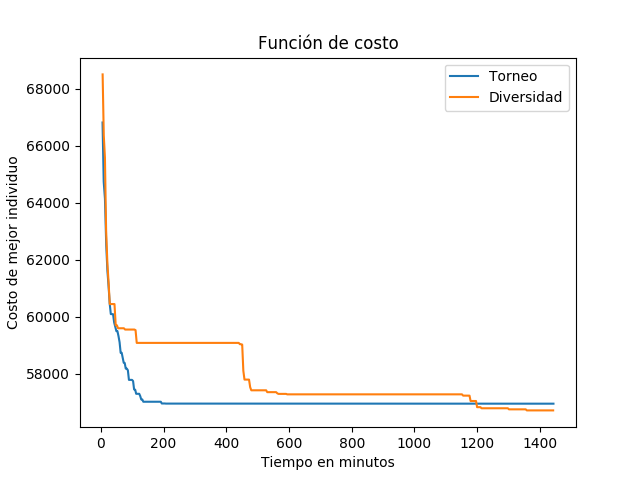
\includegraphics[scale=0.65]{1.png} 
\end{figure}

\noindent Se puede apreciar que sin un control de diversidad la mejor solución se encuentra relativamente rápido, en menos de $200$ minutos, de ahí en adelante no se obtiene una mejora; por otro lado, el progreso que tiene el algoritmo genético con control de diversidad tiene un progreso más lento, pero eventualmente llega a una mejor solución que el que no tiene control de diversidad. Si se presta atención, se puede ver que aún en los últimos minutos se tienen pequeñas mejoras.

\noindent La versión que utiliza torneo alcanza a dar $438$ generaciones y la versión que usa diversidad $398$. 

\noindent Se presenta un fenómeno que es de suma importancia en este proyecto, el control de diversidad realmente ayuda a evitar la convergencia prematura. Aquí hay al menos dos perspectivas:

\begin{enumerate}
\item[•] Implementar una versión paralela y llegar al resultado más rápido, es decir, esa solución que se encontró en $200$ minutos, quizá se pueda encontrar en un menor tiempo.
\item[•] Implementar una versión paralela que permita explorar mayor cantidad individuos en el espacio de búsqueda en diferentes regiones.
\end{enumerate}

\noindent Es bueno adquirir soluciones rápidamente, pero si de igual manera se dejará corriendo determinado tiempo el algoritmo, la segunda idea es más atractiva.

\noindent En cada estrategia, se buscó el promedio de la diferencia entre la primer mejor solución después de los $200$ minutos de ejecución y la mejor solución al terminal el programa. El promedio de la diferencia con la estrategia de torneo es de $383{.}6$ y con control de diversidad es de $1551{.}7$. Con la estrategia de torneo, en los primeros minutos se encuentran soluciones cercanas a la mejor y después la mejora es relativamente poca; en cambio, con un control de diversidad, se aprovecha mejor el tiempo de ejecución para explorar el espacio de búsqueda. Por lo anterior, solo se corre la versión paralela usando control de diversidad.

\noindent La versión paralela se ejecutó con $40$ núcleos, $20$ en un nodo $c-1-i$ y $20$ en otro nodo $c-1-j$ de \textit{El insurgente}. Como una ejecución requiere de muchos más recursos que una versión secuencial, solo se ejecutó $4$ veces la versión paralela y se utilizaron los mismos argumentos. A continuación se presenta una tabla con los resultados.

\begin{table}[H]
\centering
\begin{tabular}{|l|l|l|l|}
\hline
Estrategia & Promedio & Mínimo & Máximo \\
\hline
Torneo & 57653.7 & 56940 & 59220 \\ 
Diversidad & 57406.1 & 56704 & 57925 \\
Paralelo & 55845.2 & 55524 & 56222 \\
\hline
\end{tabular}
\end{table}

\noindent Se puede observar que la versión paralela tiene una mejora significativa con respecto a las implementaciones secuenciales. Algo agradable es que la peor mejor solución de la versión paralela es mejor que las otras dos mejores soluciones. A continuación se muestra una Figura donde se compara la función de costo en los mejores casos de las implementaciones que tienen control de diversidad.

\begin{figure}[H]
\centering
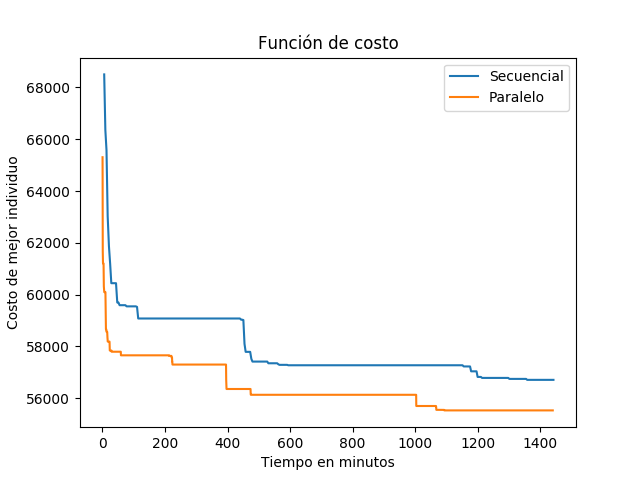
\includegraphics[scale=0.65]{2.png} 
\end{figure}

\noindent Se observa que por el minuto $400$ la versión paralela alcanza a la versión secuencial y después sigue decreciendo. Mientras la versión secuencial realizó $398$ generaciones, la versión paralela realizó $6903$, aproximadamente $17$ veces más iteraciones. 

\noindent La mejor solución encontrada en este conjunto de datos tiene un costo de $55524$, Segura et al reportan una mejor solución con costo $55339$ y un promedio de $56349$. Aunque el promedio es más bajo, la calidad de los experimentos es menor, Segura et al ejecutaron el código $30$ veces e hicieron pruebas estadísticas, en este proyecto solo se ejecutó $4$ veces la versión paralela y ninguna prueba estadística fue realizada. 

\noindent Por curiosidad, se probó con $K = 39$. Se ejecutó el programa en paralelo $4$ veces con $40$ núcleos. Se obtuvo un promedio de $9063{.}25$, donde la peor evaluación fue de $9390$ y la mejor evaluación tuvo costo $8825$. Segura et al reportan un promedio de $8567.8$ y la mejor solución encontrada con costo $55339$. Aún con experimentos más relajados, con un $K$ mayor se obtienen resultados más bajos. 

\section{Comentarios e inquietudes}

\begin{enumerate}
\item[•] Nunca había hecho ejecuciones tan largas. Aunque sabía que pasaría, me tenía nervioso que al principio los costos eran más altos con el control de diversidad que con el torneo.

\item[•] Me faltó tiempo para seguir haciendo pruebas cómodamente (con este y con otros conjuntos), parte del proyecto estuve preocupado porque tenía que terminar todo con días de anticipación para dejar corriendo los códigos un buen rato y esperar que los resultados tuvieran sentido; aunque se puede tener referencia con ejecuciones de $15$ minutos siento que no es lo mismo.

\noindent Después de pensarlo un poco, creo que podría no ser bueno que haga un torneo para reducir la población a la mitad después del torneo o la selección por diversidad. Se tendrían que hacer de nuevo los experimentos para ver si mejora o empeora pero ya no queda tiempo.

\item[•] También probé con la métrica SIM pero el control de diversidad no me cuadraba, al normalizar la distancia, esperaba que $\dfrac{0{.}75 N}{2N}$ fuera un buen valor, pero el promedio de las distancias no se mantenía arriba, cosa que sí pasaba con la distancia de Hamming, por eso terminé utilizando la distancia de Hamming. Aún así, incluyo las funciones que hice para SIM.

\item[•] Tratando de entender un poco mejor lo que pasaba, calculé distancias promedio y entropías. En ejecuciones largas, con control de diversidad ambas se mantenían en un intervalo algo alto y de momento me resulta poco intuitivo, así que terminé basándome méramente en la función de costo. Es cierto que con selección de torneo la entropía sí bajaba, pero en esta parte sentí falta de experiencia en algoritmos genéticos porque no me fue fácil interpretar lo que veía.

\item[•] Con $K= 39$ los resultados se quedan bajos, creo que ahí influye mucho la búsqueda local, pues el espacio de búsqueda es más grande. Quizá sea bueno experimentar con vecindad N2. 

\item[•] Fue interesante partir de una búsqueda aleatoria y llegar a un algoritmo memético con control de diversidad. Los pasos fueron: búsqueda aleatoria, búsqueda local, búsqueda local iterada, algoritmo memético, algoritmo memético con control de diversidad y algoritmo con control de diversidad haciendo las búsquedas locales en paralelo. A pesar de no dominar el tema de la entropía y distancias promedio, conforme se iba avanzando se iban obteniendo mejores resultados y eso me agradó.

\end{enumerate}


\end{document}